
\section{Validation case studies}\label{sec:validation} 

Here the term ``validation'' describes the comparison of numerical model output with physical observations in those cases where the observations are believed to be sufficiently-complete and of sufficient quality so that the performance of the numerical model can be assessed \cite{Roache,Wesseling}.  Roughly speaking, validation can happen when the observations or data are better than the model, so the comparison measures the quality of the numerical model and not merely errors in, or incompleteness of, the data.  Because of the difficulty of measuring boundary conditions for real ice flows, this situation is not automatic in glaciology, or even common.\footnote{This explains the rise of ``simplified geometry intercomparisons''; see section \ref{sec:simp}.}

\subsection{An SIA flow model for a table-top laboratory experiment}\label{sec:labgum}
\index{PISM!validation of SIA flow model} \index{validation!SIA flow model}

Though there are additional complexities to the flow of real ice sheets, an ice sheet is a shear-thinning fluid with a free surface.  PISM ought to be able to model such flows in some generality, and we test that ability here.

The example in this subsection compares PISM's isothermal SIA numerical model to a laboratory observations of a 1\% Xanthan gum suspension in water in a table-top moving-margin experiment by R.~Sayag and M.~Worster \cite{SayagWorster2013,SayagPeglerWorster2012}.  Their ``gum'' fluid is more shear-thinning than ice, and it has much lower absolute viscosity values, but it has the same density.  On the other hand, their flow has total mass $\sim 1$ kg, compared to $\sim 10^{18}$ kg for the Greenland ice sheet.  We compare our numerical results to their ``constant-flux'' experiment.

Figure \ref{fig:labgumexperiment} reproduces Figures 2(c) and 2(d) from \cite{SayagWorster2013}, and it shows the experimental setup.  A pump pushes the transparent, but blue-dyed, fluid through a round 8 mm hole in the middle of a flat, clear table at a mass rate of about 3 gm/s.  The downward-pointing camera, which produced the right-hand figure, allows easy measurement of the location of margin of their ``ice cap'', and in particular of its radius.  These measured radii data are the ``$\times$'' symbols in Figure \ref{fig:labgumresult} below.

\begin{figure}[ht]
\centering
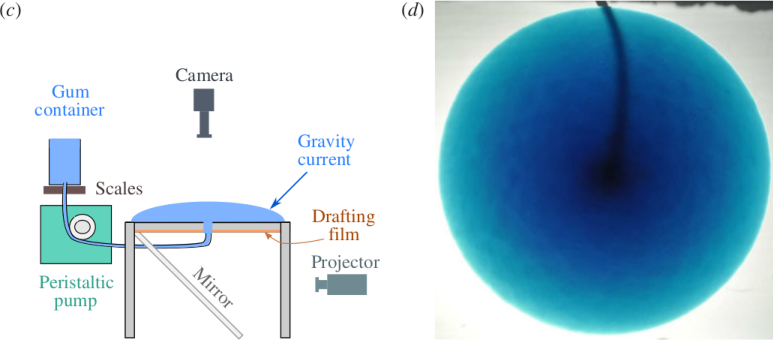
\includegraphics[width=6.0in,keepaspectratio=true]{labgumexperiment}
\caption{Reproduction of Figures 2(c) and 2(d) from \cite{SayagWorster2013}.  Left: experimental  apparatus used for ``constant-flux release'' experiment.  Right: snapshot of constant-flux
experiment (plan view), showing an axisymmetric front.}
\label{fig:labgumexperiment}
\end{figure}

The closest glaciological analog would be an ice sheet on a flat bed fed by positive \emph{basal} mass balance (i.e.~``refreeze'') underneath the dome, but with zero mass balance elsewhere on the lower and upper surfaces.  However, noting that the mass-continuity equation is vertically-integrated, we model the input flux (mass balance) as arriving at the \emph{top} of the ice sheet, as is usual for PISM.  While this represents a very large change in the vertical component of the velocity field, we will see good agreement in the overall shape of the ``ice sheet'', and specifically in the rate of margin advance.

The flow though the input hole is assumed to be constant across the hole, so the input ``climate'' has uses \texttt{-surface given} with a field \texttt{climatic_mass_balance} (in the bootstrapping file) which is a positive constant in the hole and zero outside.

Sayag \& Worster estimate Glen exponent $n = 5.9$ for the flow law of their ``gum'' fluid, using regression of laboratory measurements of the radius.  This is one of several changed-from-defaults configuration parameters, compared to PISM ice sheet defaults, which are overridden at run time by using the \texttt{-config_override} option.  See \texttt{examples/gumparams.cdl} for the settings of these parameters.

To run the example, first do
\begin{verbatim}
$ python preprocess.py
\end{verbatim}%$
and then do a run for 746 model seconds \cite{SayagWorster2013} on an 10 mm grid (520 mm / 52 subintervals) using 4 processors:
\begin{verbatim}
$ ./rungum.sh 4 53 &> out.lab53 &
\end{verbatim}%$
This run generates text file \texttt{out.lab53}, diagnostic files \texttt{ts_lab53.nc} and \texttt{ex_lab53.nc}, and final output \texttt{lab53.nc}.  The run took about 5 minutes on a 2013 laptop.

When it is done, you can compare the modeled radius to the experimental data:
\begin{verbatim}
$ ./showradius.py -o r53.png -d constantflux3.txt ts_lab53.nc
\end{verbatim}%$
You can also redo the whole thing on a higher resolution grid (here: 2.5 mm), and when that run is done after several hours, make a combined figure just like Figure \ref{fig:labgumresult}:
\begin{verbatim}
$ ./preprocess.py -Mx 209 -o initlab209.nc
$ ./rungum.sh 4 209 &> out.lab209 &
$ ./showradius.py -o foo.png -d constantflux3.txt ts_lab*.nc
\end{verbatim}%$

\begin{figure}[ht]
\centering
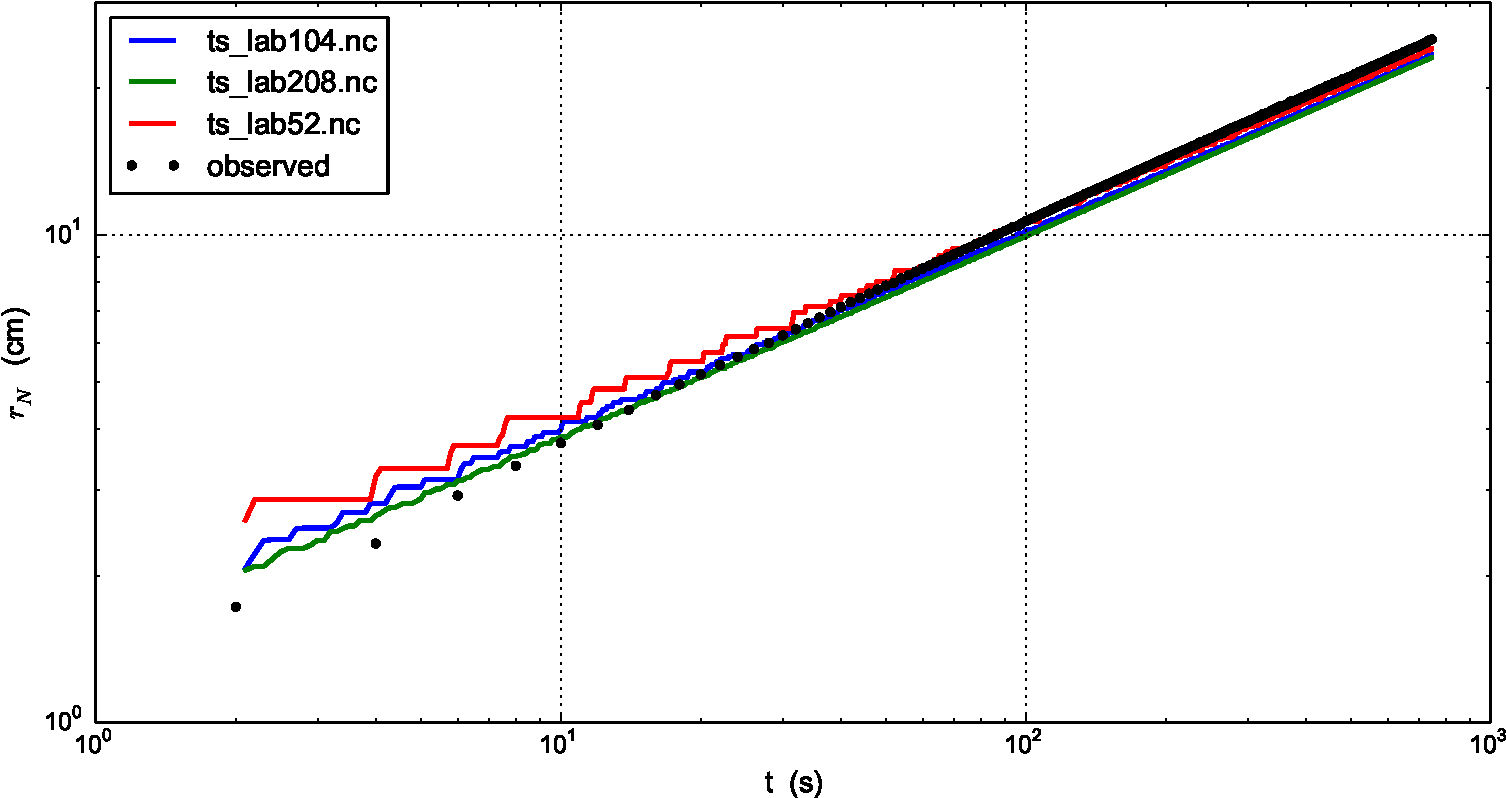
\includegraphics[width=6.0in,keepaspectratio=true]{labgumradius}
\caption{Time series for ``ice cap'' radius for runs with 10 mm (\texttt{ts_lab53.nc}) and 2.5 mm (\texttt{ts_lab209.nc}) grid spacing, compared with observations from Sayag \& Worster's \cite{SayagWorster2013} table-top experiment with gravity current a 1 \% Xanthan gum suspension.}
\label{fig:labgumresult}
\end{figure}

Results are distinctly better on finer grids because the input hole has radius of only 8 mm.  Furthermore the ``ice cap'' has radius comparable to the hole for the first few model seconds.  The early evolution is distinctly non-shallow, but resolution makes most of the difference.  In fact, we know there is little need for ``higher-order'' stresses because the exact similarity solution, with a point source, used by Sayag \& Worster, closely-fits the data even for small radius and time \cite[Figure 4]{SayagWorster2013}.  In any case, the large-time observations are closely-fit by the numerical results at all grid resolutions.


\subsection{An SSA flow model for the Ross Ice Shelf in Antarctica}\label{sec:ross} \index{PISM!diagnostic Ross ice shelf model}\index{Ice Sheets!Antarctic ice sheet!Ross ice shelf} \index{PISM!validation of SSA ice shelf model}\index{validation!SSA ice shelf model} \index{Ross ice shelf}
\optsection{Ross ice shelf}

As part of the EISMINT series of intercomparisons, MacAyeal and others \cite{MacAyealetal} validated several ice shelf numerical models using velocity data for the Ross ice shelf.  The data were from RIGGS survey \cite{RIGGS2}, acquired in the period 1973--1978 and measured at a few hundred locations in a grid across the shelf.  Substantial modelling developments followed EISMINT-Ross, including inverse modeling to recover depth-averaged viscosity \cite{RommelaereMacAyeal} and parameter-sensitivity studies \cite{HumbertGreveHutter}.  Previous PISM versions set up the EISMINT-Ross flow model and performed the diagnostic computation, with RIGGS data for validation.  However, increased availability of data sets for ice sheet modeling, including the public ALBMAP v1 \cite{LeBrocqetal2010} geometry and climate data set and the MEaSUREs InSAR-Based Antarctica Velocity Map \cite{Rignotetal2011}, allow us to use more complete, recent, and higher-resolution data.

The scripts in this subsection are found in the directory \texttt{examples/ross/}.  In summary, the script \texttt{preprocess.py} downloads data and builds a NetCDF input file for PISM.  The script \texttt{run.sh} runs PISM.  The script \texttt{plot.py} shows a comparison of observations and model results, as in Figure \ref{fig:rosspython}.


\subsubsection*{Grabbing the data}

Our setup uses geometry and surface boundary condition data from the ALBMAP and surface velocity from MEaSUREs.  (See \texttt{preprocess.py} for URLs of these data.)  We use NetCDF Operators to cut out the relevant portion of the grid and CDO to conservatively-interpolate high-resolution (500 m) velocity data onto the coarser (5 km) geometry grid used in ALBMAP.  The script \texttt{nc2cdo.py}, included in the PISM distribution in directory \texttt{util/}, prepares the NetCDF file for the application of CDO, which requires complete projection information.  Run

\begin{verbatim}
$ python preprocess.py
\end{verbatim}%$

The NetCDF file \texttt{Ross_combined.nc} produced by \texttt{preprocess.py} contains ice thickness, bed elevations, surface temperature, net accumulation, as well as latitude and longitude values.  All of these are typical of ice sheet modeling data, both in evolution and diagnostic runs.

The file also has variables \texttt{u_ssa_bc} and \texttt{v_ssa_bc} for the boundary values used in the (diagnostic) computation of velocity.  They are used at all grounded locations and ice shelf cells that are immediate neighbors of grounded ice.  The variable \texttt{bcflag} specifies these locations.


\subsubsection*{Diagnostic computation of ice shelf velocity}
A diagnostic Ross ice shelf velocity computation from these data initializes from \texttt{Ross_combined.nc} and does a zero-year run:

\begin{verbatim}
$ mpiexec -n 2 pismr -boot_file Ross_combined.nc \
          -Mx 211 -My 211 -Mz 21 -Lz 3000 -z_spacing equal \
          -stress_balance ssa -energy none -yield_stress constant -tauc 1e6 -pik \
          -ssa_dirichlet_bc -y 0 -o out_211.nc -o_order zyx
\end{verbatim}%$
The computational grid here is the ``native'' $5$ km data grid used in ALBMAP.  The maximum thickness of the ice is $2766$ m so we choose a height for the computational box large enough to contain the ice (i.e.~``\texttt{-Lz 3000}'').  There is no need to type in the above command; just do

\begin{verbatim}
$ ./run.sh 2
\end{verbatim}%$

\noindent Several command-line options require explanation:
\begin{itemize}
\item \texttt{-stress_balance ssa} selects the SSA stress balance and
  turns off the SIA stress balance computation, since our goal is to
  model the ice shelf. It also side-steps a technical issue: PISM uses
  periodic boundary conditions at domain boundaries and most fields in
  this setup are not periodic. Turning off SIA avoids operations such
  as differencing surface elevation across the domain edges. For a
  more complete solution to this technical issue see section
  \ref{sec:jako} on a regional model using option
  \verb|-no_model_strip| and executable \verb|pismo|.
\item \texttt{-ssa_dirichlet_bc} reads fields \texttt{u_ssa_bc}, \texttt{v_ssa_bc}, \texttt{bcflag}, and \texttt{thk} from an input file and uses them to prescribe Dirichlet boundary conditions for the SSA velocity (\texttt{u_ssa_bc} and \texttt{v_ssa_bc} are components of the SSA B.C., \texttt{bcflag} is $1$ at B.C. locations and $0$ elsewhere) and \texttt{thk} at $\mathtt{bcflag} = 1$ locations is used as the Dirichlet B.C. condition for the ice thickness. The latter (together with Dirichlet B.C. for the SSA velocity) can be thought of as prescribing ``SSA ice flux'' at given locations in an \emph{evolution} run.
\item \texttt{-yield_stress constant -tauc 1e6} sets the constant high yield stress. In this setup the selected yield stress value is irrelevant, because SSA velocities at grounded locations are prescribed.
\item \texttt{-pik} enables PIK improvements (see section \ref{sec:pism-pik}). The most important one here is the calving front stress boundary condition (CFBC), option \verb|-cfbc|.
\item \texttt{-y 0} makes PISM stop after the first one-model-second-long ``preliminary'' time-step.  The model state is reset after this time-step, making it equivalent to a ``diagnostic'' run.
\end{itemize}

The script \texttt{run.sh} allows changing grid resolution and using the SSA flow law enhancement factor as a tuning parameter.  There are many reasonable choices of tuning parameters, and using an enhancement factor acknowledges that the physical justification for tuning is uncertain.  One could instead use ice softness in an isothermal setup, or temperature in a thermomechanically-coupled setup, for example.  Even the density of the ice shelf might be used as a tuning parameter, because high accumulation rates and cold firn, and basal freeze-on of marine ice, may generate significant changes in shelf density.

The script \texttt{plot.py} takes PISM output such as \texttt{out_211.nc} to produce Figure \ref{fig:rosspython}.  The run shown in the figure used an enhancement factor of $0.6$.  The thin black line outlines the floating shelf, which is the actual modeling domain here.  To generate your own, do

\begin{verbatim}
$ python plot.py out_211.nc
\end{verbatim}%$

\begin{figure}[ht]
\centering
\mbox{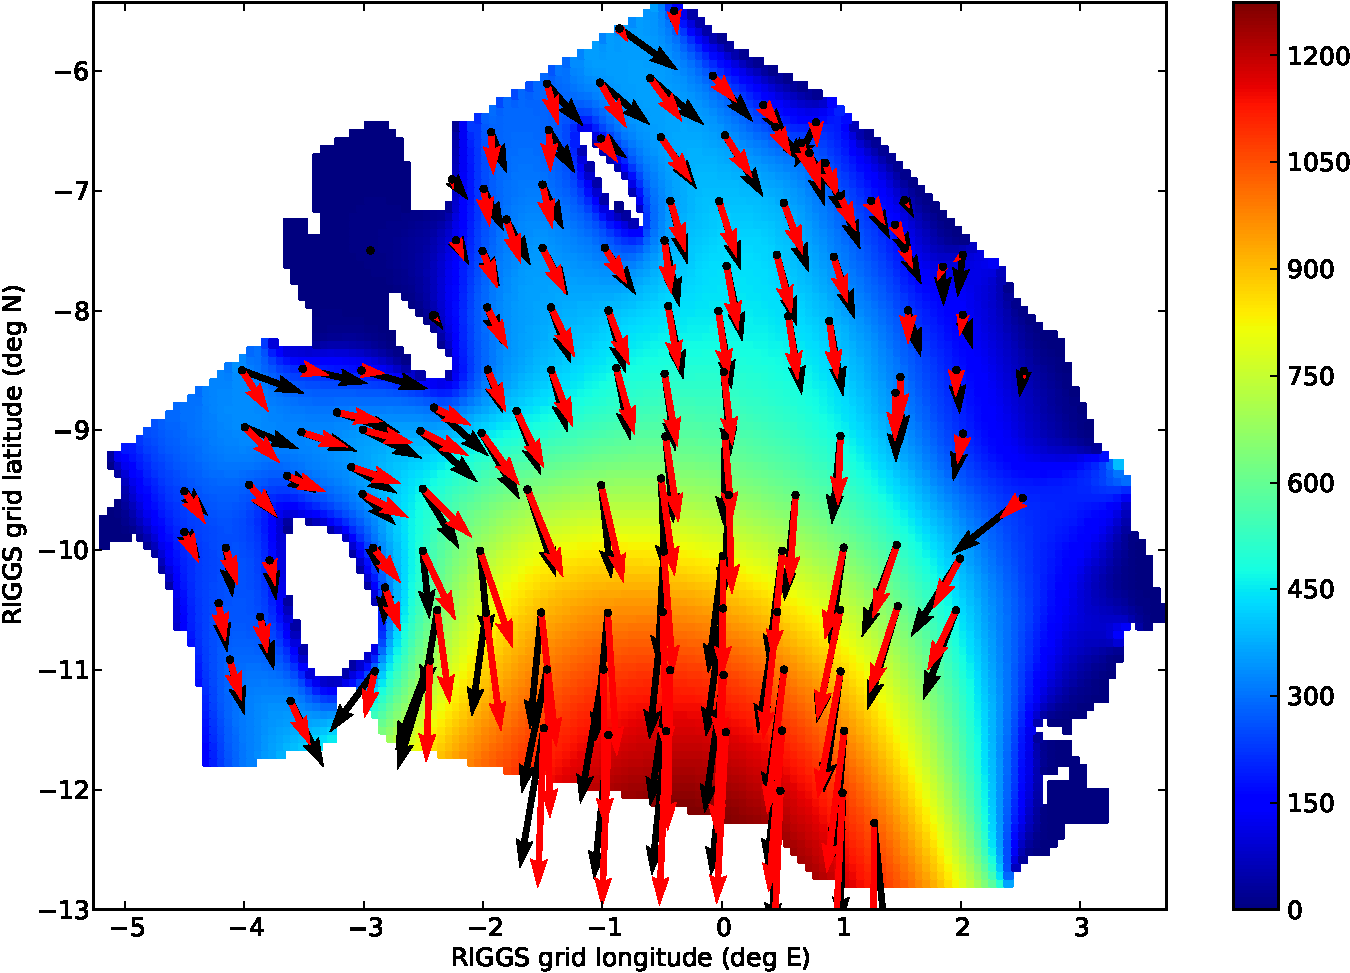
\includegraphics[width=3.3in,keepaspectratio=true]{rossquiver}\quad 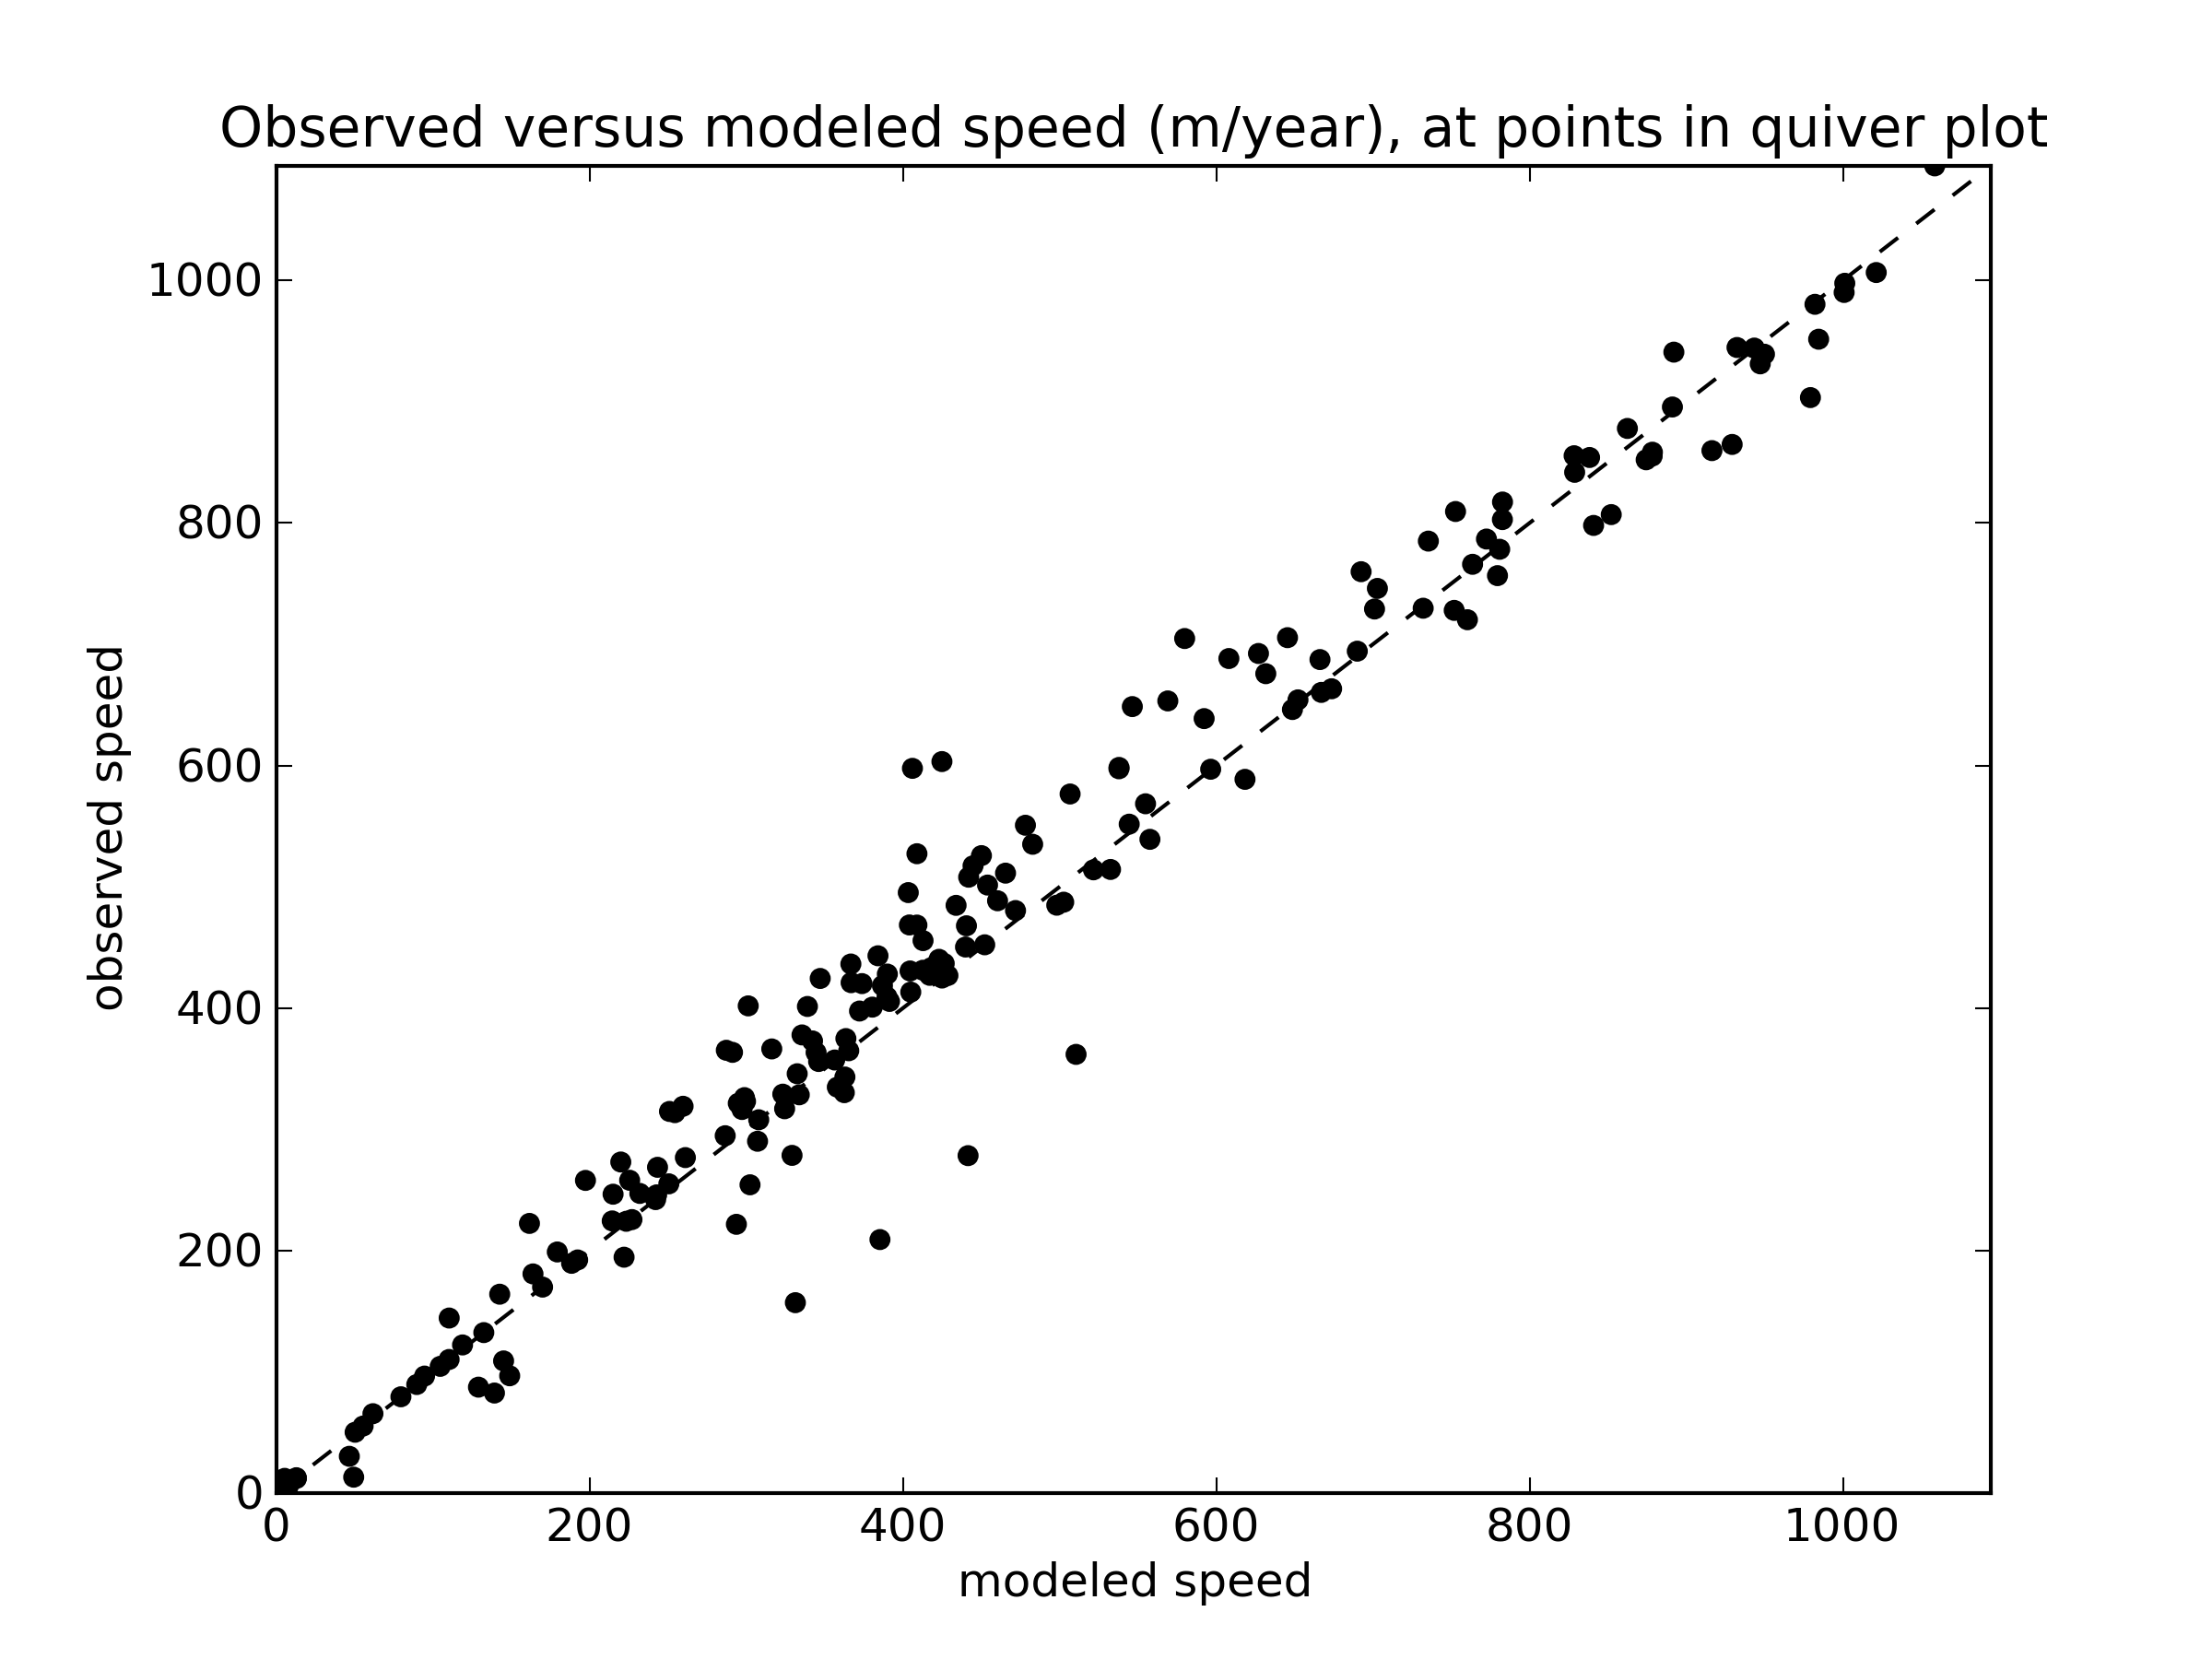
\includegraphics[width=2.7in,keepaspectratio=true]{rossscatter}}
\caption{\protect{\emph{Left}}: Color is speed in m/a.  Arrows are observed (white) and modeled (black) velocities.  \protect{\emph{Right}}: Comparison between modeled and observed speeds at points plotted on the left.}
\label{fig:rosspython}
\end{figure}

\subsubsection*{Extending this example}

\begin{itemize}
\item \textbf{Other ice shelves.}  The SSA solution described in this section can be easily applied to other ice shelves in Antarctica, including the Filchner-Ronne Ice Shelf as in \cite{AlbrechtLevermann2012}, for example.  All you need to do is to choose a different rectangular domain (within the area covered by the whole-ice-sheet data-sets used here).  In particular you should modify the line ``\texttt{ncks -O -d x1,439,649 -d y1,250,460 ...}'' in \texttt{examples/ross/preprocess.py}.
\item \textbf{Prognostic (geometry-evolving) runs.}  One can also create an evolving geometry model of an ice shelf with constant-in-time inflow across the fixed grounding line.  See \texttt{README.md}, \texttt{preprocess_prog.py}, and \texttt{run_prog.sh} in \texttt{examples/ross/prognostic/}.  This example demonstrates the \intextoption{eigen_calving} model for a moving calving front \cite{Levermannetal2012}.
\item \textbf{Evolving fracture density.}  See \texttt{README.md}, \texttt{preprocess_frac.py}, and \texttt{run_frac.sh} in directory \texttt{examples/ross/fracture_density/}.  This example demonstrates the fracture density transport model in \cite{AlbrechtLevermann2012}.
\end{itemize}

%%% Local Variables:
%%% mode: latex
%%% TeX-master: "manual"
%%% End:
